\chapter{Conclusion}
\label{conclusion}

\section{Contribution}
In this dissertation, I focus on the critical HCI question of how to encourage drivers to follow unselfish routes for their daily commutes. I explored motivational techniques that support making informed decisions during navigation towards unselfish, purposeful, and effective driving behaviors. 

As someone who is not a driver, I began with an observational study of drivers using modern navigation applications in their daily commutes. I found that while drivers choose a recommended route in urgent situations, many still preferred to follow familiar routes. They also made deviations from their original choice because of unfamiliar roads, lack of local context, perceived driving unsuitability, and inconsistencies with realized navigation experiences. Here, I argue that we should rethink our longstanding assumptions and mental models about drivers and navigation tools which are limiting the progress of navigation tools. Instead of treating drivers as docile actors, designers should instead support their self-efficacy and agency in performing navigation tasks. Navigational applications are only as good as the data it senses and estimates from models. While we are still far from having near accurate navigational information, designers should explore visualizing uncertainty and missing data on maps and other sections of the application. Modern navigation applications, like Google Maps and Waze, passively collect GPS data and other trip information to improve their maps and routing algorithms. Designers should maximize this information and provide true personalization in terms of route recommendations and voice guidance. In relation to personalization, designers should also consider maximizing the embedded social networks in applications. We learned from the results that aside from trusting what is already familiar to them, drivers also trust information coming from their close contacts, especially those living near their destinations. 

I continue this line of research by designing and evaluating two separate techniques that aim to help drivers make better informed navigation decisions. Both are informed by the Self-Determination Theory. The first is a GUI-based approach that focuses on the trip planning phase of a driving task. Using Self-Determination Theory, I show how the simple addition of motivative and familiarity information can help navigation applications positively encourage the use of unselfish routes. Through route choice experiments and pairwise comparisons, all combinations of motivative and familiarity information were able to convince drivers to choose the unselfish route at least once. Specifically, drivers were most likely to choose the unselfish route when a simple positive framing is used along with a list of familiar roads. Aside from the effectiveness of simple and explicit motivational and familiarity information, results also showed that drivers with moderate impersonal and controlled orientation need more support for relatedness. Thus, information that emphasizes social comparison would be more effective. The use of motivational and familiarity information shows the potential of navigation applications as a civic technology, transforming it to empower positive societal impact. 

En route to a destination, traffic conditions along a chosen route might change or there might be alternative routes the are worthy to discover. The second voice-based technique explores the use of two-party conversations between voice agents in giving alternative turns or routes. I show how designers of navigation applications can slowly move away from designing voice guidance as authoritative figures that drivers would have no choice but to rely on. Indeed, results suggest that two-party conversations were able to convince drivers to follow alternative routes as they are made available. This is especially true when the alternative route is appropriate for the trip scenario. Additionally, having a point of comparison allowed drivers to reflect better on their choices, possibly affecting future choices. However, designers must still be careful in using voice-based techniques as it can increase experienced workload especially during time-constrained navigational maneuvers and turns. This voice-based technique contributes to an understanding of how navigation voice guidance and voice UIs and assistants, more broadly, can be suggestive while still respecting the agency and self-efficacy of a user or driver. It adds to the potential of designing voice guidance that are autonomy-supportive for the driver.

Addressing the shortcomings of the first two techniques while also leveraging on their strengths, my final contribution is the design and evaluation of Navigo, a holistic technique that motivates the selection of an unselfish route and encourages drivers to keep following it towards a destination, covering the whole driving navigation task. Similar to the first two techniques, Self-Determination Theory was used in providing personality-targeted motivative and familiarity information to encourage unselfish choices. In its evaluation, there is  supporting evidence that the showing the list of familiar roads and positively framing the benefits of an unselfish route choice can encourage drivers to choose unselfish routes before the start of a trip. Additionally, providing these information frequently to drivers sustained their unselfish choice in succeeding trips. Navigo also provides personality-targeted two-party conversations when a driver decides to follow an optimal route at the beginning. The conversational technique was successful in encouraging drivers to switch into following an unselfish route when they have diverse experiences of following different route choices. When the drivers choose the unselfish route at the beginning, the voice-based technique provides motivative messages along the trip. It was successful in encouraging drivers to stick to following unselfish routes. Participants liked being reminded about the positive societal benefits of their decision.

Finally, my dissertation hopes to challenge the rigidity of existing navigation application designs and hope my contributions can serve as conversation starters towards a reimagining for future designs. To build navigation applications that caters to the idiosyncratic needs of drivers while reducing its negative externalities in the communities where they operate, it is worth looking into how we can include diverse stakeholders into the co-design of such applications and their algorithms to safeguard and balance the interest of everyone.

\section{Future Directions}

Altogether, the research projects in my dissertation offer a different take as to how navigation applications can be redesigned to balance the needs of drivers and the greater sociotechnical system where they move about. While I have always envisioned my approaches to offer positive societal effects, it remains to be seen whether a widespread adoption of these solutions can actually make a difference in our road networks and encourage behavior change among drivers.

As a first future direction, I plan to move on to the actual implementation and field test of my approaches. My evaluations have always been in driving simulators with hypothetical scenarios so I am really looking forward to realize them into tangible products. I also want to explore other behavior change techniques and provide them in different modalities. For example, how can we incorporate familiarity information on the map alongside other traffic-related information? Although motivational and familiarity information can easily be provided as text, drivers still prefer exploring route choices visually, using interactive maps. 

Second, I am also excited to go back to some of the design implications in my very first study, and start working towards their fruition. Navigation applications incorporate model predictions in the traffic information they display. I want to explore how we can properly display uncertain and decaying information in maps so that everything is transparent to the driver. In the same vein, I am also excited to explore how these uncertain and decaying information can be sonified and incorporated into voice guidance for eyes-free access to crucial information.

\begin{figure}[h]
\centering
  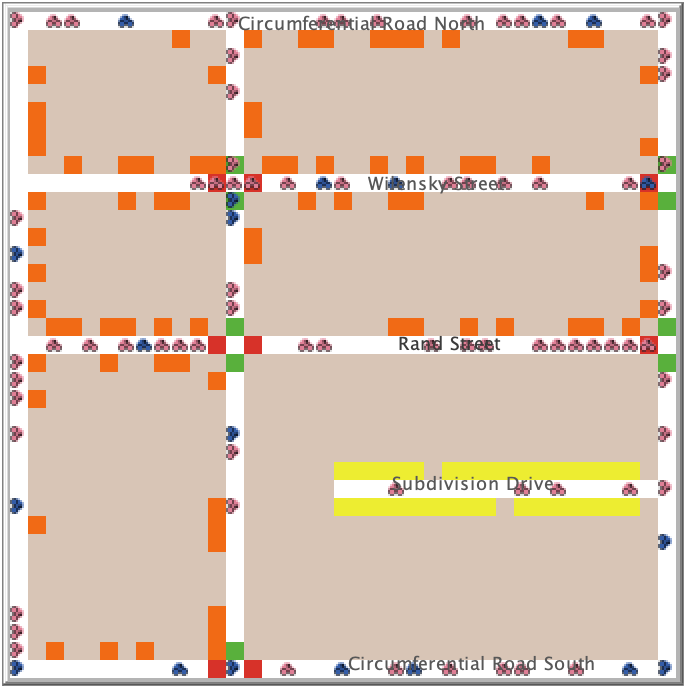
\includegraphics[scale=.8]{figures/conclusion-abm.png}
  \caption{An initial prototype of an agent-based model of drivers that follow navigation applications. It shows the effects on the traffic flow when a certain percentage of them follow the navigation applications completely. Cars that follow navigation applications are colored pink while those that do not are colored blue. Each have unique origins and destinations. Origins are indicated by the yellow boxes while destinations are in orange. Traffic lights are also present in the model.}~\label{fig:abm}
\end{figure}

Lastly, I would like to emphasize that navigation applications are not operating in a vacuum and they do not only benefit an individual user. As a sociotechnical system, it is part of a feedback loop. It adapts its recommendations based on the state of the road network, and as drivers try to follow recommendations, it indirectly affects the future state of the road network. Currently, user and lab studies are primary methods in evaluating the usability and effectiveness of HCI solution prototypes. However, in the case of sociotechnical systems like social networking platforms, online communities, and navigation applications, there is a gap in evaluating how it affects the overall system and its stakeholders. Moving forward, I plan to develop an agent-based model that simulates a simple road network in which a certain percentage of the drivers are using navigation applications. I already created an initial prototype of the model as shown in Figure \ref{fig:abm}. By incorporating the route choice and navigation behaviors found in my previous works, my goal is to evaluate how the deployment of such prototypes can have mesoscopic and macroscopic effects on the system. Ultimately, I want to develop an evaluation framework that HCI and CSCW researchers can use to evaluate their proposed technological solutions for large sociotechnical systems, without the need of a large field study which can be costly.